\documentclass[11pt]{article}
\usepackage[margin=1in]{geometry}
\usepackage{amsmath,amssymb,amsthm}
\usepackage{booktabs}
\usepackage{graphicx}
\usepackage[normalem]{ulem}
\usepackage{xcolor}
\usepackage[hidelinks]{hyperref}
\usepackage{natbib}
\usepackage{microtype}
\usepackage{placeins}
\usepackage[font=small,labelfont=bf,labelsep=period,skip=6pt]{caption}
\renewcommand{\topfraction}{0.9}
\renewcommand{\bottomfraction}{0.8}
\renewcommand{\textfraction}{0.1}
\renewcommand{\floatpagefraction}{0.75}
\setcounter{topnumber}{3}
\setcounter{totalnumber}{4}

\newcommand{\NumCells}{51}
\newcommand{\NumImproved}{33}
\newcommand{\NumMatched}{18}
\newcommand{\NumWorse}{0}
\newcommand{\MeanGain}{17.9}
\newcommand{\MaxGain}{34.1}
\newcommand{\TopCell}{$10\times13$}
\newcommand{\TopOld}{240.6}
\newcommand{\TopNew}{158.6}
\newcommand{\NumImprovedOneMin}{33}


\title{Simple Local Search Sets \NumImproved{} New Records\\for Balanced Latin Rectangles}
\author{Zhengyu Li\\ Georgia Institute of Technology\\ \texttt{brian.li@gatech.edu}
  \and Vijay Ganesh\\ Georgia Institute of Technology\\ \texttt{vganesh45@gatech.edu}}
\date{}

\begin{document}
\maketitle

\begin{abstract}
A $k\times n$ Latin rectangle is \emph{balanced} when every pair of symbols has the same total
distance, summed over the rows. The \emph{imbalance} measures how far a rectangle is from this
ideal. Field experiments in agronomy use minimum-imbalance Latin rectangles, and finding them is
a benchmark for constraint programming, SAT, and LLM-generated streamliners combined with
mixed-integer programming. We show that plain simulated annealing finds rectangles at least as
good as all published ones, and better ones on most instances. The search uses an $O(n)$ swap move and an adaptive penalty for column
conflicts. It improves the best known imbalance on \NumImproved{} of the \NumCells{} non-square
instances with $8\le n\le 13$ from the literature, and it matches the other \NumMatched{}. The
improvements average \MeanGain\% and reach \MaxGain\% (\TopCell: \TopOld{} $\to$ \TopNew). The
search is also faster by orders of magnitude. On one laptop core, it beats each previous record
after a median of \MedianBeat{} CPU seconds over \NumSeeds{} seeds, and every run beats it within
\MaxBeat{} seconds. The previous records came from pipelines that run for at least four hours per
instance. For four rectangles, a SAT approach reports solving times from 32 minutes to 5.5 hours.
Our search matches each of them in at most \MaxMatch{} seconds. We release all rectangles, an
independent checker, and the code. The new values are upper bounds, and optimality remains open
for every improved instance.
\end{abstract}

\section{Introduction}

Latin squares and rectangles are classical tools of experimental design. In a field trial,
spatial autocorrelation can bias a Latin layout when some pairs of treatments are always planted
closer together than others~\citep{vanEs1993}. \emph{Spatially balanced} Latin squares remove
this bias, because every pair of symbols has the same total
distance~\citep{GomesSellmann2004,LeBrasGomesSelman2012}. \citet{DiazLeBrasGomes2017} extended
the idea to $k\times n$ rectangles. Balanced rectangles exist only in restricted cases. Díaz et
al.\ therefore defined the \emph{imbalance} of a rectangle and asked for rectangles of minimum
imbalance. They found this optimization problem hard for CSP, local-search and MIP methods, and
they proposed it as a benchmark.

Two recent studies attacked this benchmark. \citet{RamaswamySzeider2023} used SAT encodings,
which also certify optimality with DRAT proofs. \citet{VoborilRamaswamySzeider2025} used
streamliners generated by large language models (LLMs) and evaluated them with Gurobi. This
approach improved the best known values on most open instances. Balanced Latin rectangles also
serve as a test problem for LLM agents that reformulate constraint models~\citep{VoborilSzeider2026}.

\paragraph{Contribution.} We revisit the problem with a deliberately simple method. It is
simulated annealing~\citep{KirkpatrickGelattVecchi1983} over rows that are permutations, with a
swap move that costs $O(n)$ time to evaluate. A penalty for repeated symbols in a column adapts
its weight during the search, in the spirit of strategic oscillation~\citep{GloverHao2011}. None
of these ingredients is new. Our contribution is the outcome. We call the best known value of an
instance before this work its \emph{record}. On the instances of
\citet{VoborilRamaswamySzeider2025}, our search improves \NumImproved{} of the \NumCells{}
records and is never worse. It is also fast. On a single laptop core, it beats each record after
a median of \MedianBeat{} seconds, whereas the previous pipelines run for hours per instance. We
release every rectangle with an independent checker, so anyone can check each record in seconds
without trusting our solver.

We see two consequences. First, the records on this benchmark were much further from optimal
than they appeared. This matters to anyone who uses them to judge new methods. Second, new
methods for this problem, including LLM-based ones, need a well-engineered local search as a
baseline, and not only an exact solver with a time limit.

\section{Problem}

A $k\times n$ Latin rectangle ($k\le n$) is a $k\times n$ array over the symbols
$\{1,\dots,n\}$ in which no symbol repeats in a row or in a column. Write $c_i(u)$ for the
column of symbol $u$ in row $i$. Following \citet{RamaswamySzeider2023}, the distance of two
symbols and the imbalance of $L$ are
\[
  d(u,v) = \sum_{i=1}^{k} |c_i(u)-c_i(v)|, \qquad
  I(L) = \sum_{1\le u<v\le n} \Bigl| d(u,v) - \tfrac{k(n+1)}{3} \Bigr| .
\]
The target $k(n+1)/3$ is the average of $d(u,v)$ over all pairs, because every row contributes
$\sum_{u<v}|c_i(u)-c_i(v)| = (n+1)n(n-1)/6$. The value $3I(L)$ is always an integer. As in the
literature, we write imbalances as $x.0$, $x.3$ and $x.6$ for $x$, $x+\tfrac13$ and
$x+\tfrac23$. The goal is a rectangle of minimum imbalance for given $k$ and $n$.

\section{Method}

\paragraph{Search space and move.} The state is $k$ permutations of the symbols, one per row. We
fix the first row to the identity. This loses no generality, because a relabelling of the
symbols does not change the imbalance. A move picks a row $i\ge 2$ and two columns
$j_1\ne j_2$, and it swaps the symbols $a=L[i][j_1]$ and $b=L[i][j_2]$. Rows stay permutations,
but the swap can create a repeated symbol in a column.

\paragraph{Incremental evaluation.} We keep the matrix $D$ of all pair distances. A swap in row
$i$ moves only $a$ and $b$. So only the $2(n-2)$ distances $d(a,x)$ and $d(b,x)$ with
$x\notin\{a,b\}$ change, and $d(a,b)$ stays the same. For each such $x$, with $p_x=c_i(x)$,
\[
  d'(a,x) = d(a,x) - |j_1-p_x| + |j_2-p_x|, \qquad d'(b,x) = d(b,x) - |j_2-p_x| + |j_1-p_x|.
\]
The search therefore computes the exact change of $3I(L)$ in $O(n)$ integer operations. A
recomputation from scratch costs $O(kn^2)$.

\paragraph{Column conflicts.} Let $V$ be the number of excess symbol occurrences over all
columns. Per-column counters give $V$ in $O(1)$ time per move. The search minimizes
$3I(L) + W\cdot V$, and it records only rectangles with $V=0$. The weight $W$ starts at $k$.
Every $2^{16}$ moves, the search multiplies $W$ by $1.02$ if the current state has conflicts and
by $0.99$ if it has none, and it clamps $W$ to $[1, 4n^2]$. The penalty matters most when $k$ is
close to $n$. There, almost every swap creates a conflict, so a search that effectively forbids
conflicts stalls. Our first version used a large fixed penalty ($W=4n^2$). In 10-second runs on
$6\times7$ and $7\times7$, it never visited a conflict-free rectangle other than its start. With
the adaptive weight, 20-second runs reach the known optima of both instances (20.0 and 18.6).

\paragraph{Annealing schedule.} The search starts from the cyclic rectangle
$L[i][j]=i+j \bmod n$. It accepts a move with change $\Delta$ if $\Delta\le 0$, and otherwise
with probability $e^{-\Delta/T}$. The temperature $T$ starts at $T_0=2k$ and falls by a factor of
$0.9999995$ after every move, with a floor of $0.05$. When the best rectangle does not improve
for $4\cdot 10^{7}$ moves, the search resets $T$ to $T_0$. Each run is single-threaded and stops
after a fixed CPU time. Before it reports its best rectangle, it recomputes the imbalance from
scratch. The implementation has about 130 lines of C.

\section{Experiments}

\paragraph{Setup.} We use the instances in Table~1 of \citet{VoborilRamaswamySzeider2025}, with
$8\le n\le 13$ and $2\le k\le n-1$. This gives \NumCells{} instances. We omit squares ($k=n$),
because different structure governs that case~\citep{XiaEtAl2026}. The record of each instance is
the best value reported there. It already includes earlier results and four-hour Gurobi runs. We
used an Apple M3 laptop (8 cores, 16\,GB) and ran eight single-threaded runs at a time. Each
instance got one run with a budget of 1 minute and one run with 5 minutes, with different seeds.
The larger instances ($k\ge4$, $n\ge9$) also got one 10-minute run. We report the best rectangle
per instance, so no instance used more than 16 CPU minutes.

\paragraph{Verification.} An independent Python program checks every reported rectangle. We wrote
it from the definition above. It uses exact rational arithmetic and shares no code with the
solver. To make sure that it computes the published quantity, we ran it on all eleven
rectangles printed in~\citep{RamaswamySzeider2023,VoborilRamaswamySzeider2025}. These include the
eight CP 2025 records of their Figure~6, up to $12\times13$. The checker reproduces every reported
imbalance exactly.

\paragraph{Results.} Table~\ref{tab:results} shows the outcome. The
search improves \NumImproved{} instances, matches \NumMatched{}, and is worse on \NumWorse. All
improved instances have $n\ge 9$ and $k\ge 3$. The search matches the record on all instances
with $n=8$ or $k=2$, on all instances with $k=3$ except $3\times12$, and on $4\times10$,
$5\times10$ and $6\times12$. Several of these records are proven
optimal~\citep{RamaswamySzeider2023}. The gains grow with the size of the instance
(Figure~\ref{fig:records}a), up to \MaxGain\% for \TopCell. The one-minute runs alone beat the
record on \NumImprovedOneMin{} instances. Longer runs mainly widen the margin. Over the
\NumBudgetCells{} instances that got all three budgets, the mean reduction relative to the record
is \BudgetOneMin\% after one minute, \BudgetFiveMin\% after five minutes and \BudgetTenMin\%
after ten minutes.

\begin{table}[tb]
\centering
\small
\begin{tabular}{rccccccccccc}
\toprule
$n \backslash k$ & 2 & 3 & 4 & 5 & 6 & 7 & 8 & 9 & 10 & 11 & 12 \\
\midrule
8 & 40.0 & 36.0 & 32.0 & 30.0 & 24.0 & 28.0 &  &  &  &  &  \\[2pt]
9 & 65.3 & 56.0 & \shortstack{\textbf{53.3}\\{\tiny\sout{56.0}}} & \shortstack{\textbf{48.6}\\{\tiny\sout{52.6}}} & \shortstack{\textbf{40.0}\\{\tiny\sout{48.0}}} & \shortstack{\textbf{43.3}\\{\tiny\sout{51.3}}} & \shortstack{\textbf{42.6}\\{\tiny\sout{53.3}}} &  &  &  &  \\[2pt]
10 & 92.0 & 80.0 & 78.6 & 66.6 & \shortstack{\textbf{60.0}\\{\tiny\sout{70.0}}} & \shortstack{\textbf{58.0}\\{\tiny\sout{72.0}}} & \shortstack{\textbf{58.6}\\{\tiny\sout{82.6}}} & \shortstack{\textbf{64.0}\\{\tiny\sout{70.0}}} &  &  &  \\[2pt]
11 & 124.0 & 114.0 & \shortstack{\textbf{104.0}\\{\tiny\sout{112.0}}} & \shortstack{\textbf{94.0}\\{\tiny\sout{116.0}}} & \shortstack{\textbf{88.0}\\{\tiny\sout{108.0}}} & \shortstack{\textbf{84.0}\\{\tiny\sout{118.0}}} & \shortstack{\textbf{78.0}\\{\tiny\sout{114.0}}} & \shortstack{\textbf{84.0}\\{\tiny\sout{120.0}}} & \shortstack{\textbf{100.0}\\{\tiny\sout{110.0}}} &  &  \\[2pt]
12 & 168.0 & \shortstack{\textbf{152.0}\\{\tiny\sout{154.0}}} & \shortstack{\textbf{149.3}\\{\tiny\sout{154.6}}} & \shortstack{\textbf{140.0}\\{\tiny\sout{145.3}}} & 120.0 & \shortstack{\textbf{121.3}\\{\tiny\sout{164.0}}} & \shortstack{\textbf{116.6}\\{\tiny\sout{148.0}}} & \shortstack{\textbf{106.0}\\{\tiny\sout{154.0}}} & \shortstack{\textbf{124.0}\\{\tiny\sout{174.6}}} & \shortstack{\textbf{136.6}\\{\tiny\sout{147.3}}} &  \\[2pt]
13 & 218.6 & 198.0 & \shortstack{\textbf{201.3}\\{\tiny\sout{211.3}}} & \shortstack{\textbf{191.3}\\{\tiny\sout{210.6}}} & \shortstack{\textbf{166.0}\\{\tiny\sout{204.0}}} & \shortstack{\textbf{164.0}\\{\tiny\sout{203.3}}} & \shortstack{\textbf{160.0}\\{\tiny\sout{220.6}}} & \shortstack{\textbf{152.0}\\{\tiny\sout{214.0}}} & \shortstack{\textbf{154.6}\\{\tiny\sout{240.6}}} & \shortstack{\textbf{168.0}\\{\tiny\sout{224.0}}} & \shortstack{\textbf{166.0}\\{\tiny\sout{274.0}}} \\[2pt]
\bottomrule
\end{tabular}

\caption{Best known imbalance of $k\times n$ Latin rectangles. Bold: new value from this work,
with the record~\citep{VoborilRamaswamySzeider2025} struck through below it. Plain: record that
our search matches.}
\label{tab:results}
\end{table}

\paragraph{Speed.} To measure speed directly, we ran the search on every improved instance with
\NumSeeds{} further seeds. Each run stopped as soon as its imbalance fell below the record, with
a cap of five CPU minutes (Figure~\ref{fig:records}b). All \NumTimingRuns{} runs beat the record.
The median time is \MedianBeat{} seconds, and the slowest run took \MaxBeat{} seconds. The
median per instance is below one second on \NumCellsUnderOneSec{} of the \NumImproved{}
instances. It is below one minute on all of them, with a maximum of \MaxCellMedian{} seconds
for $9\times10$. For comparison, each approach of \citet{VoborilRamaswamySzeider2025} runs for 4
to 9 hours per instance, after a 4-hour Gurobi baseline. They also report that their
incremental warmstart approach is still 25--60\% worse than the baseline after one minute.

\begin{figure}[tb]
\centering
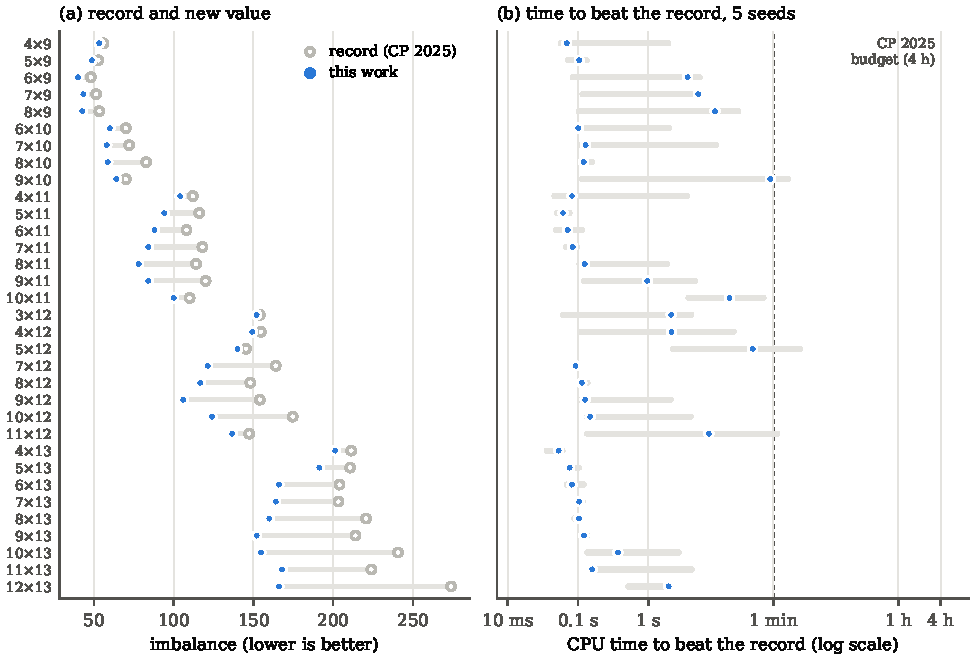
\includegraphics{../figures/records_speed.pdf}
\caption{All \NumImproved{} improved instances. (a)~Record (open circle) and new imbalance
(filled). (b)~CPU time until the search beats the record, on one core: median (dot) and range
(bar) over \NumSeeds{} seeds, log scale. The dashed lines mark one minute and one 4-hour run of
one CP 2025 approach.}
\label{fig:records}
\end{figure}

\citet{RamaswamySzeider2023} report the SAT solving time for four rectangles that set records at
that time. The times range from 32 minutes ($3\times10$, imbalance 84) to 5.5 hours
($6\times11$, imbalance 124). Figure~\ref{fig:speedsat} shows all four. In every run, our search
reaches the same imbalance within \MaxMatch{} seconds. By the median, it is at least
\MinSpeedupSAT{} times faster.

\begin{figure}[tb]
\centering
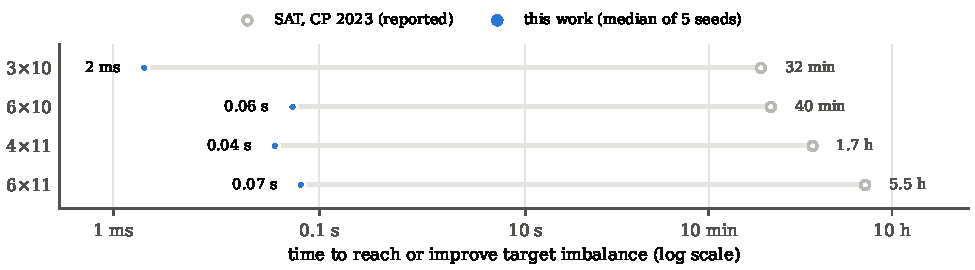
\includegraphics{../figures/speed_cp2023_paper.pdf}
\caption{Time to find a rectangle with the imbalance that the SAT approach
of~\citet{RamaswamySzeider2023} reports, next to its reported solving time. Ours: median of
\NumSeeds{} seeds. Log scale.}
\label{fig:speedsat}
\end{figure}

\section{Discussion}

\paragraph{Why does a simple method do so well?} We have not tested this, but the structure of
the problem suggests an explanation. The objective is a sum of $\binom n2$ absolute deviations. A
MIP model must linearize every one of them. Its LP relaxation can make all pairs look nearly
balanced at once, so it likely gives the solver little guidance. Streamliners help the solver
because they restrict it to a structured subspace, but the best rectangles need not lie in that
subspace. Local search avoids both problems. The search updates the objective exactly and
cheaply, the swap neighbourhood is natural, and the penalty lets the search cross infeasible
states. The problem suits annealing unusually well, and we do not claim that the comparison
carries over to other problems.

\paragraph{What this means for LLM-based methods.} The previous records came from a pipeline that
combines Gurobi, five LLMs and an evolutionary search over streamliners. This pipeline runs for
hours per instance. A simulated-annealing search of about 130 lines of C improves
\NumImproved{} of these records and matches the other \NumMatched{}, within seconds. We do not
read this result as a verdict on LLM-generated streamliners. Their goal is generality across
constraint models, not the best solver for one problem. A general method can lose to a
specialized one on a single benchmark. We do read the result as a reminder about baselines.
Local search for balanced Latin designs goes back at least to \citet{SmithGomesFernandez2005},
and \citet{DiazLeBrasGomes2017} included it among their methods. Yet the two recent studies of
this benchmark~\citep{RamaswamySzeider2023,VoborilRamaswamySzeider2025} compare only against
exact solvers and earlier records. New methods for this benchmark, LLM-based or not, should
report a strong problem-specific baseline next to the exact solvers.

\paragraph{How fair is the speed comparison?} The gap spans four to five orders of magnitude, so
we state its caveats plainly.
\begin{enumerate}
\item The hardware differs. The earlier work used Intel Xeon E5-2640~v4 servers from 2016. We
used an Apple M3 laptop from 2023. Its single-core speed is higher by a small factor, not by
orders of magnitude.
\item CP 2025 does not report when within its runs it found each record. We therefore compare our
time to beat a record with the length of their runs, not with their time to reach the record.
\item The CP 2023 times come from a complete SAT solver on a decision encoding. These instances
are satisfiable, so the solver had to find a rectangle, which is the same task as ours. Its
encoding, however, is built to prove infeasibility as well.
\item We did not rerun either pipeline ourselves.
\end{enumerate}
Together, these caveats are unlikely to explain a gap of this size.

\paragraph{Limitations.} The new values are upper bounds. We prove nothing about optimality, and
the size of the improvements suggests that the remaining gap to the optimum may still be large.
The final records come from one run per instance and budget. Only the speed experiment uses
several seeds. Finally, the benchmark stops at $n=13$, and larger instances are an obvious next
step.

\section{Conclusion}

A short, standard simulated-annealing search improves \NumImproved{} of the \NumCells{} best
known imbalance values for balanced Latin rectangles in the recent literature, and it matches
the rest. It beats each record within seconds on a laptop, where earlier methods ran for hours
on a server. Natural next steps follow from this.
\begin{itemize}
\item Prove lower bounds or optimality for the improved instances, for example with the SAT
approach of \citet{RamaswamySzeider2023}.
\item Extend the benchmark to larger instances.
\item Compare exact, LLM-guided and local-search methods on equal hardware.
\end{itemize}

\paragraph{Data and code.} Rectangles, checker, solver and scripts:
\url{https://github.com/BrianLi009/Balanced-Latin-Rectangles}.

\FloatBarrier
\bibliographystyle{plainnat}
\bibliography{refs}

\end{document}
